%
%  Chapter:  2 - Nuclear Models for High Spin Phenomena
%  Modified: 2/16/2015
%  Author:   James Till Matta
%
%%%%%%%%%%%%%%%%%%%%%%%%%%%%%%%%%%%%%%%%%%%%%%%%%%%%%%%%%%

\chapter{NUCLEAR MODELS FOR HIGH SPIN PHENOMENA}
\label{chp:models}

\section{Introduction}
\label{sec:models-into}
The atomic nucleus, discovered in $1911$ by Ernest Rutherford \cite{rutherfordNuclearModel}, is a tiny point of matter at the heart of an atom. The nucleus is approximately $1-10fm$ across, contains more than $99.94\%$ of an atom's mass and is composed of protons and neutrons. Additionally, the nucleus has a powerful short range force that overcomes the Coulomb repulsion to produce a bound system. This force's range is quite limited, perhaps nearest neighbors only as can be seen in the saturation of binding energy per nucleon around $A\sim60$ at a value close to $8.5$MeV.

\begin{figure}[h!]
\centerline{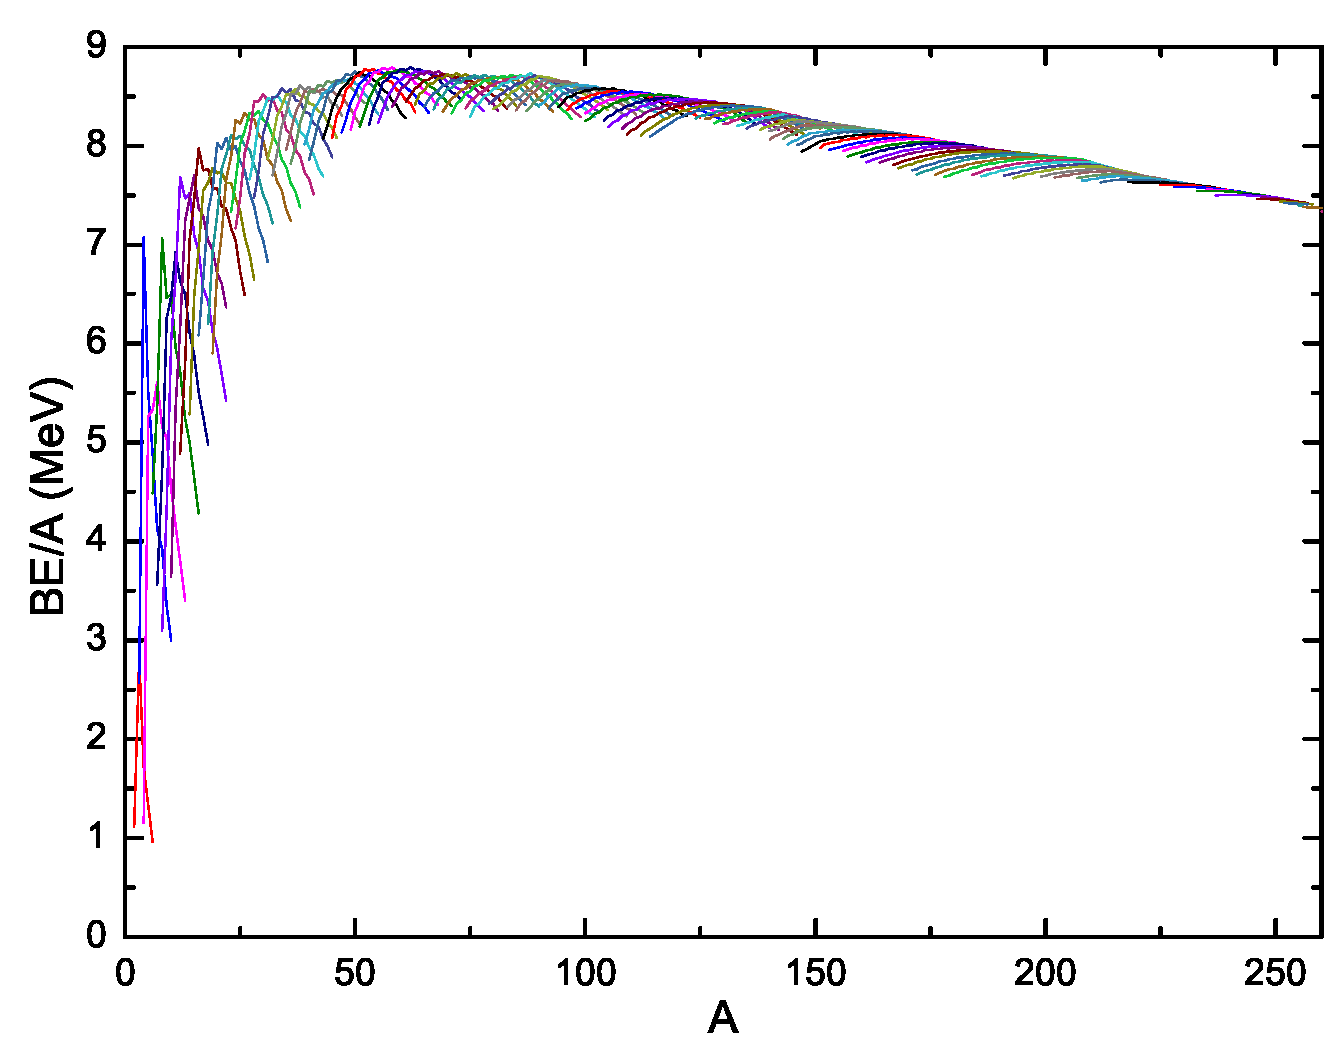
\includegraphics[width=\textwidth]{./img/c2/binding_plot.eps}}
	\caption{Binding energies per nucleon plotted versus mass number. Values calculated from: Ref.\cite{AME20031,AME20032}\label{fig:chp2-binding}}
\end{figure}

Examination of the two proton and two neutron separation energies (Fig \ref{fig:chp2-masses}) shows several distinct discontinuities at specific numbers of protons or neutrons. Further examination of the energies of the first $2^+$ (Fig \ref{fig:chp2-two-plus-energies}) states show peaks at the same numbers. These ``Magic Numbers'' occur at numbers of protons and neutrons where there is a dramatic drop off in the nucleus' stability with the addition of another nucleon. Further evidence for magic numbers of protons and neutrons can be found in the near zero quadrupole moments of nuclei located at these magic numbers, substantially decreased neutron absorption cross-sections at neutron magic numbers, and enhanced abundance for nuclides where N and Z are magic numbers. The magic numbers are $2$, $8$, $20$, $28$, $50$, $82$, and $126$, with $40$ and $64$ also weakly magic over certain ranges of N and Z.

\begin{figure}[h!]
\centerline{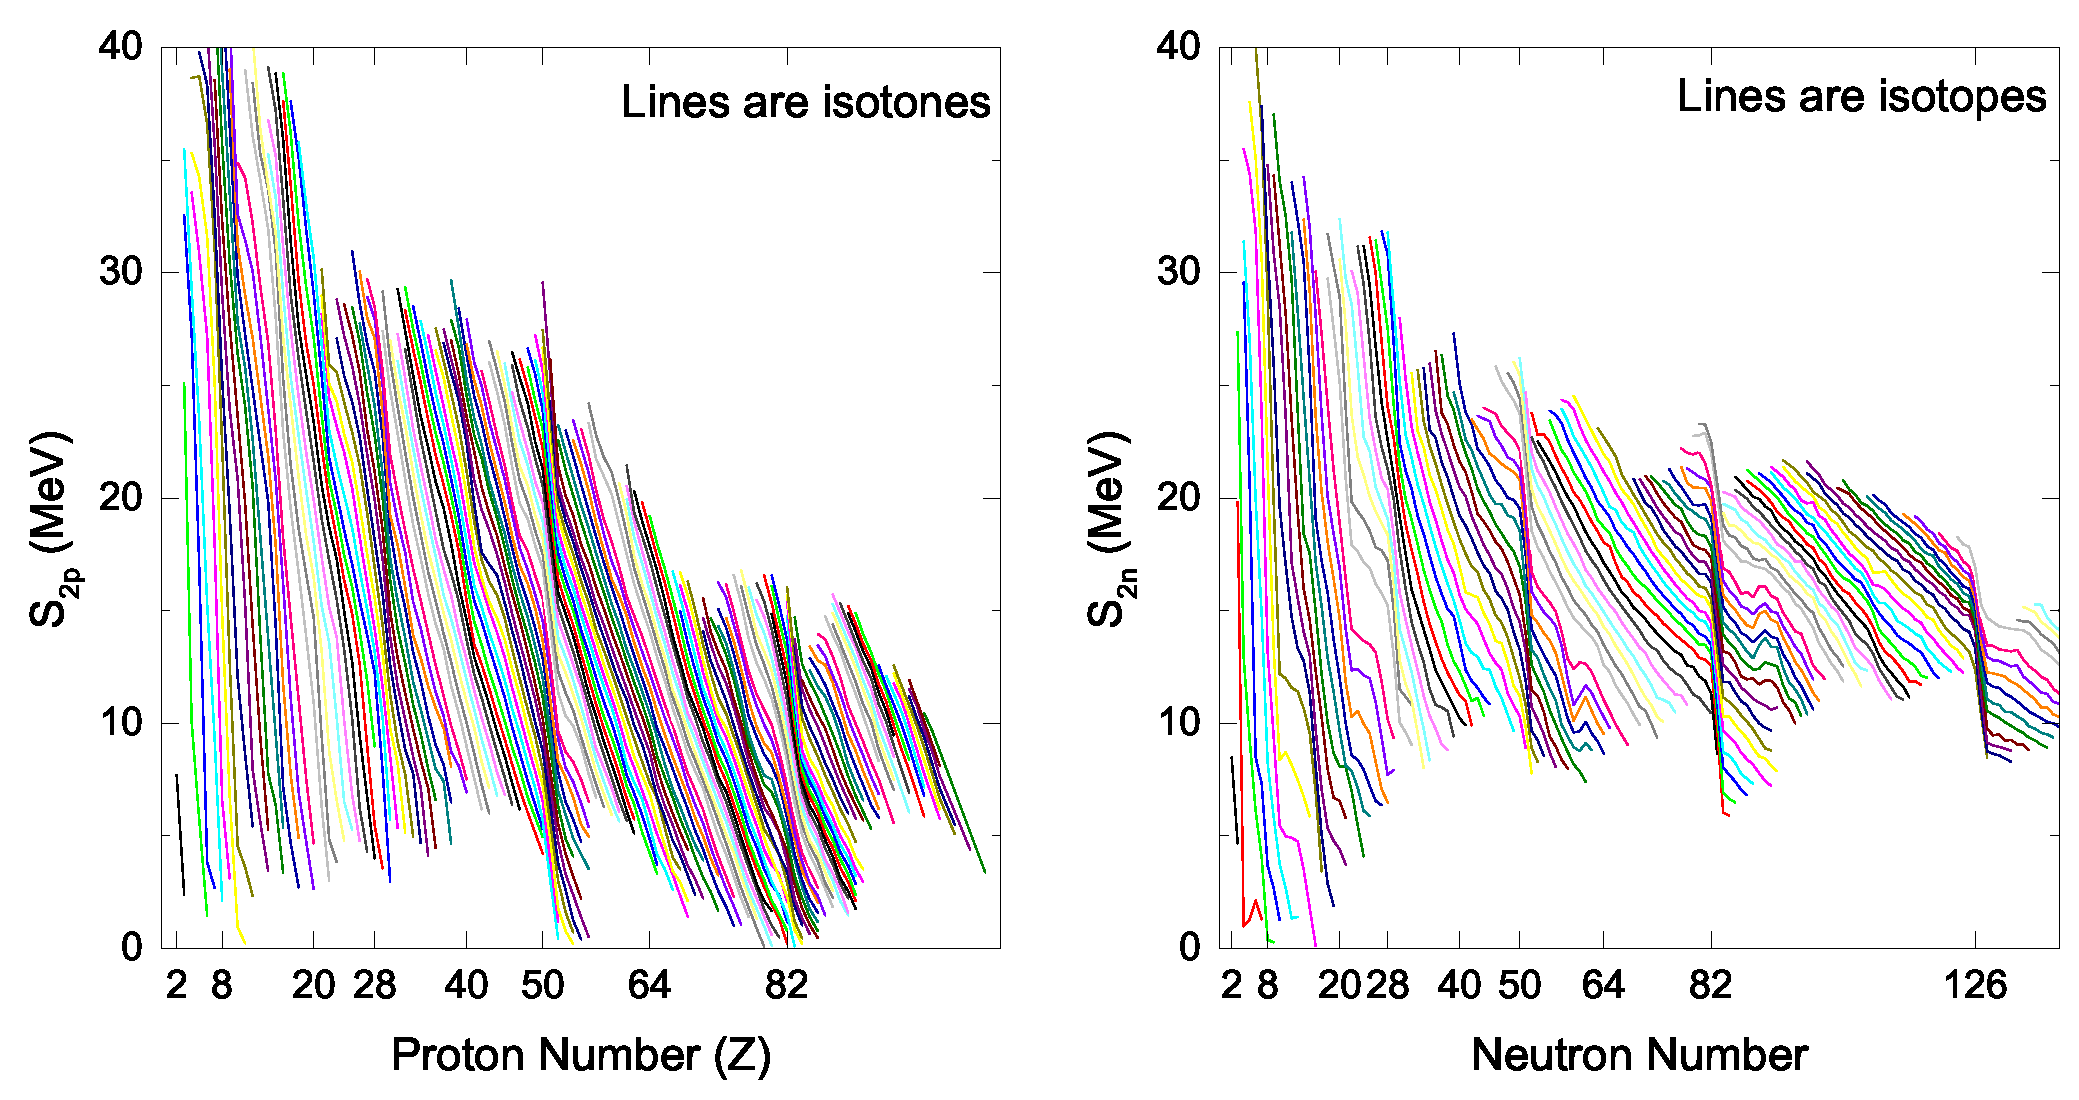
\includegraphics[width=\textwidth]{./img/c2/2nuc_sep_en.eps}}
	\caption{Left: Two proton separation energies plotted versus proton number. Each line is a set of isotones. Right: Two neutron separation energies plotted versus neutron number. Each line is a set of isotopes. Values calculated from: Ref.\cite{AME20031,AME20032}\label{fig:chp2-masses}}
\end{figure}

\begin{figure}[h!]
\centerline{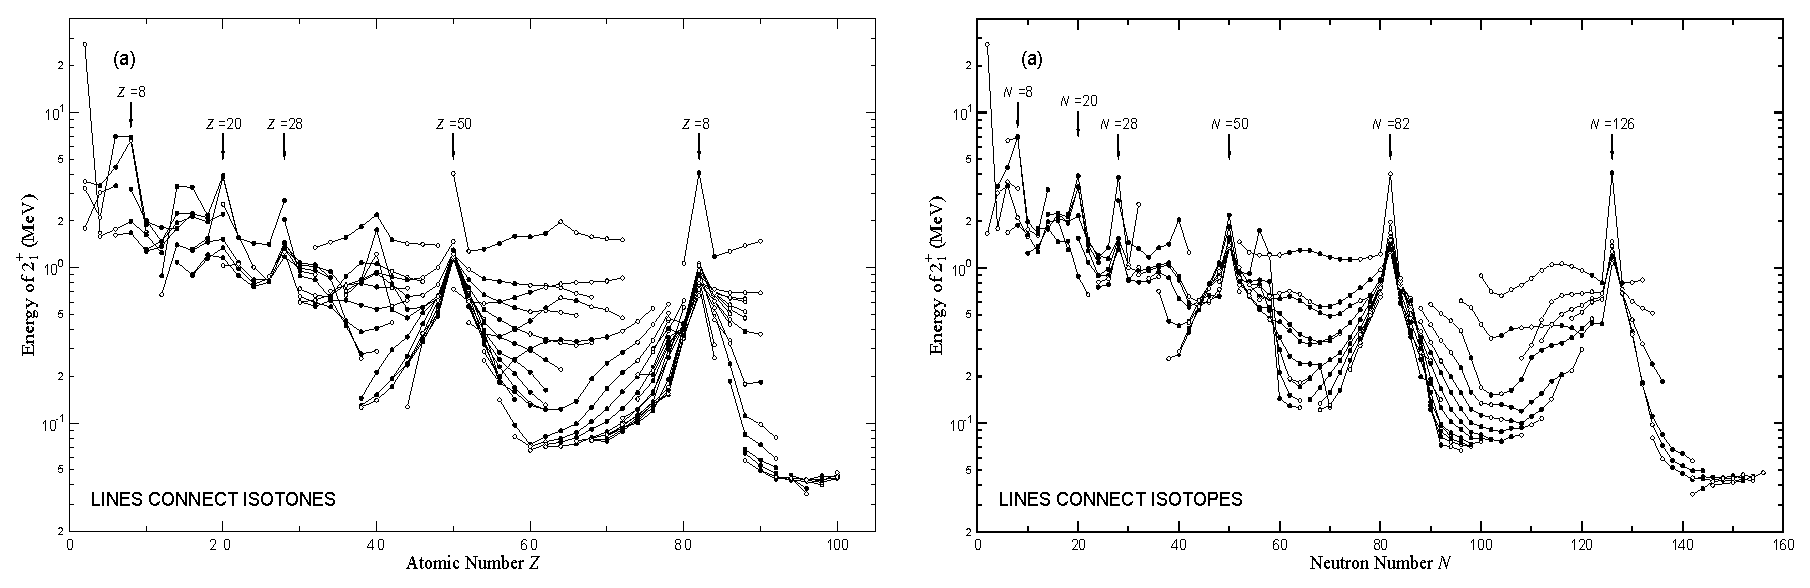
\includegraphics[width=\textwidth]{./img/c2/2_plus_en.eps}}
	\caption{Left: First excited $2^+$ energies of nuclei with even Z and N, plotted versus proton number. Each line is a set of isotones. Right: First excited $2^+$ energies of nuclei with even Z and N, plotted versus neutron number. Each line is a set of isotopes. Figures adapted from: Ref.\cite{RamanTwoPlus}\label{fig:chp2-two-plus-energies}}
\end{figure}

Analogy to atomic theory reveals these magic numbers are major shell closures. This leads to the conclusion that the nucleus has shell structure, leading to the shell model of the nucleus. These numbers can be derived from the calculation of a single particle in a mean field potential. A caveat on these magic numbers is that, far from stability, quenching of the know shell gaps and the opening of new shell gaps has been observed \cite{changingShells}.

Contrariwise, in seeming contradiction to the preceding analogy to atomic theory, the nucleus also exhibits collective excitations such as rotation and vibration which are described later in the chapter. The crucial difference between an atomic system and the nuclear system lies in its occupation of the shells with two types of particles, protons and neutrons. With this, certain shell occupation can lead to the ``single particle behavior'' exhibited around closed shells, while a different occupation can yield collective phenomena.

\section{The Shell Model}
\label{sec:models-shell-model}
The nuclear shell model, in its simplest incarnation, seeks to explain the shell structure observed in nuclei by describing them and independent particles in a mean field potential produced by the other nucleons. While the short range nature of the nuclear force might lead one to use a square well potential or similar as the mean field, the Simple Harmonic Oscillator (SHO) potential is a reasonable first order approximation (seen in Figure \ref{fig:chp2-SHOPot}), which happens to be much simpler to solve. Placing a single particle in the SHO potential gives the first few magic numbers observed; however, to reproduce all the magic numbers it is necessary to add a centrifugal $\vec{l}^2$ potential and a strong spin-orbit ($\vec{l}\cdot\vec{s}$ potential. The Hamiltonian for such a potential is as follows:
\begin{equation}
\label{eqn:chp2-sm-sho-hamil}
\mathbf{\mathit{H}} = \frac{-\hbar^2}{2m}\nabla^2 + \frac{1}{2}m(\omega r)^2 + \beta \uvec{l}^2 + \alpha \uvec{l}\cdot{}\uvec{s}
\end{equation}
The progression of shell gaps from $SHO$ to $SHO + \vec{l}^2$ to $SHO + \uvec{l}^2 + \uvec{l}\cdot\uvec{s}$ is shown in Figure \ref{fig:chp2-shell-model}.

\begin{figure}
\label{fig:chp2-SHOPot}
\centerline{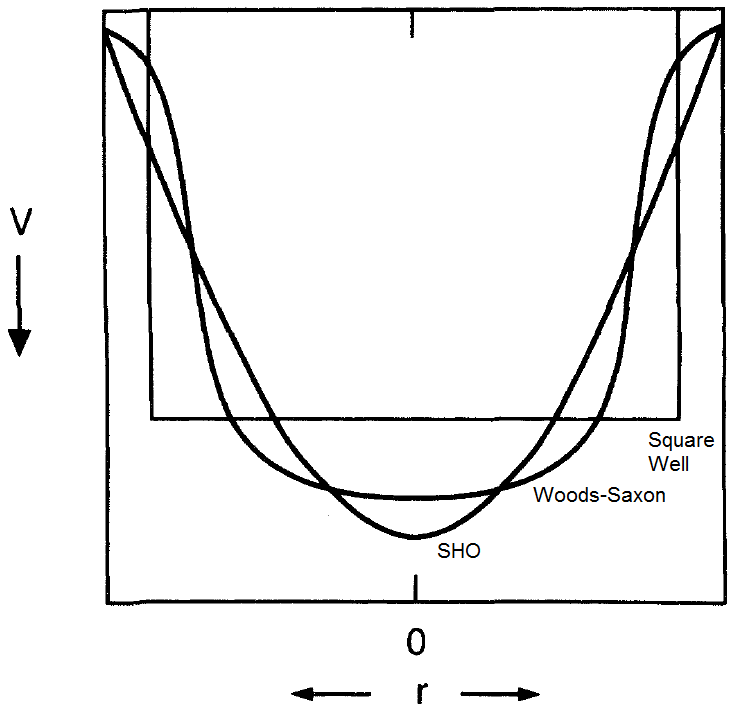
\includegraphics[height=0.25\textheight]{./img/c2/sho_approx.png}}
	\caption{Schematic of a square well, SHO potential, and a realistic Woods-Saxon potential. Figure adapted from: Ref.\cite{casten}}
\end{figure}

\begin{figure}
\label{fig:chp2-shell-model}
\centerline{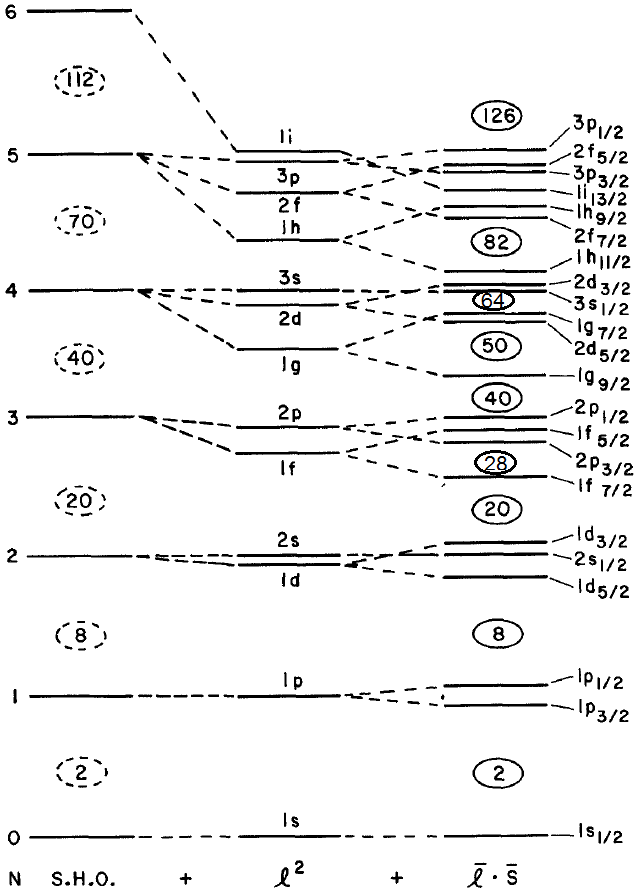
\includegraphics[height=0.45\textheight]{./img/c2/shell_model.png}}
	\caption{Spectrum of a single nucleon in an SHO potential, SHO + centrifugal potential, and, finally, SHO + centrifugal + spin-orbit. Figure adapted from: Ref.\cite{casten}}
\end{figure}

TODO: Talk about quantum numbers and the like

In more realistic shell model calculations the SHO potential is discarded and a Woods-Saxon potential is adopted. Here the Hamiltonian becomes:
\begin{equation}
\label{eqn:chp2-sm-ws-hamil}
\mathbf{\mathit{H}} = \frac{-\hbar^2}{2m}\nabla^2 + \frac{V}{1+e^{(r-R)/a}} - \alpha(r)\uvec{l}\cdot\uvec{s}
\end{equation}
where $R=r_0A^{1/3}$, $r_0\sim1.2$fm, $a\sim0.5$fm, and $V\sim50$MeV. In addition to the Woods-Saxon component, a spin orbit term is again necessary to reproduce the observed shell gaps. The central flatness of the Woods-Saxon potential mimics the saturation of the nuclear force better than an SHO potential. This increased realism comes at the cost of increase difficulty in calculations and the loss of quantum numbers, in this model the only good quantum numbers are $J=\mathit{l}+\mathit{s}$ and $\pi = (-1)^\mathit{l}$.

Until this point, the nucleons were considered as independent particles with in a mean field which was the average potential produced by the other particles. This description, while powerful, is not accurate, especially for nuclei away from the closed shells. The missing piece is the interactions between nuclei that are not accounted for in the mean field, often called ``residual interactions''. Residual interactions must be accounted for to produce an accurate description of the nucleus.

\section{The Deformed Shell Model}
\label{ssec:models-shell-model-def-sm}
\subsection{Parameterization of Deformation}
In the standard shell model the potentials are spherically symmetric, depending only on the radius. While this is a successful approach near the shell gaps where nuclei are spherical, or nearly spherical, this breaks down in the deformed regions further from shell closures. In such nuclei, the effective long-range forces experienced by the valence nucleons can lead to deformation as the valence nucleons are arranged into deformed shells with lower energy levels. When the nuclear shape is deformed the surface of the nucleus is described with a parametric function defining the radius as follows:
\begin{equation}
\label{eqn:surface-full-expansion}
R(\theta, \phi) = R_{o}\left \lgroup 1 + \sum_{\lambda = 2}^{\infty}\sum_{\mu = -\lambda}^{\lambda}\alpha_{\lambda \mu} Y_{\lambda \mu}(\theta, \phi)\right \rgroup
\end{equation} 
Here $R_0$ is the radius of a sphere with the same volume as the deformed nucleus, $Y_{\lambda \mu}(\theta, \phi)$ are the spherical harmonic functions, and $\alpha_{\lambda \mu}$ are the coefficients of the expansion. The expansion starts at $\lambda = 2$ because the $\lambda = 1$ corresponds to the translation of the center of mass, a term easily eliminated by requiring the nuclear center of mass to coincide with the coordinate's origin. The first of the non-trivial terms, $\lambda = 2$, corresponds to the components of quadrupole deformation, $\lambda = 3$ gives octupole deformation, $\lambda = 4$ gives hexadecapole deformation, so on and so forth. As $\lambda = 2$ is the most important component in this work, only quadrupole deformation terms will be considered from this point on.

The quadrupole shapes cover oblate spheres (two semi-major axes, like a pumpkin), prolate spheres (two semi-minor axes, like an American football), and triaxial shapes (all three axes are different lengths, like a potato). To preserve spheroidal symmetry $R(\theta,\phi) = R(\pi - \theta,-\phi)$ the five quadrupole shape parameters are reduced to two independent parameters $a_{2 0}$ and $a_{2 2}$, with the conditions: $a_{2 -2}=a_{2 2}$ and $a_{2 1}=a_{2 -1}=0$. Further, it is common to parameterize the remaining expansion coefficients using the Hiller-Wheeler variables, $\beta$ and $\gamma$, as follows \cite{wongBook}:
\begin{align}
\label{eqn:chp2-hiller-wheeler}
a_{2 0} = \beta Cos(\gamma)  & &  a_{2 2} = a_{2 -2} = \frac{1}{\sqrt{2}}\beta Sin(\gamma)
\end{align}
Expanding the spherical harmonics as:
\begin{align}
\label{eqn:spherical-harmonics}
Y_{2 0}(\theta, \phi) &= \frac{1}{4} \sqrt{\frac{5}{\pi }} \left(-1+3 Cos(\theta )^2\right)\\
Y_{2 2}(\theta, \phi) &= \frac{1}{4} e^{2 i \phi } \sqrt{\frac{15}{2 \pi }} Sin(\theta)^2\\
Y_{2 -2}(\theta, \phi) &= \frac{1}{4} e^{-2 i \phi } \sqrt{\frac{15}{2 \pi }} Sin(\theta)^2
\end{align} 
and inserting all this into Equation \ref{eqn:surface-full-expansion} yields:
\begin{equation}
\label{eqn:quadrupole-surface}
R(\theta, \phi) = R_{o}\left(1+\sqrt{\frac{5}{16 \pi }}\beta  \left(Cos(\gamma ) \left(3 Cos(\theta )^2-1\right)+\sqrt{3} Sin(\gamma ) Sin(\theta )^2Cos(2 \phi ]\right)\right)
\end{equation} 
The Hiller-Wheeler variables have some redundancy, for $\beta>0$ the nucleus is prolate for $\gamma=0^{\circ},120^{\circ},240^{\circ}$ and oblate for $\gamma=180^{\circ},300^{\circ},60^{\circ}$. However, for $\gamma=0^{\circ}$ and $\gamma=180^{\circ}$ the symmetry axis is the $\uvec{z}$-axis of the intrinsic frame, for $\gamma=120^{\circ}$ and $\gamma=300^{\circ}$ the symmetry axis is the $\uvec{x}$-axis, and for $\gamma=240^{\circ}$ and $\gamma=60^{\circ}$ the symmetry axis is the $\uvec{y}$-axis. The Lund convention makes use of this redundancy by establishing the following rules \cite{wongBook}:
\begin{enumerate}
\item $\beta\geq0$
\item For rotation about the smallest axis $0^{\circ}\leq\gamma\leq60^{\circ}$
\item For rotation about the longest axis $-120^{\circ}\leq\gamma\leq-60^{\circ}$
\item For rotation about the intermediate axis $-60^{\circ}\leq\gamma\leq0^{\circ}$
\end{enumerate}
A graphical schematic of the Lund convention is in Figure \ref{fig:chp2-lund}
\begin{figure}[t!]
\label{fig:chp2-lund}
\centerline{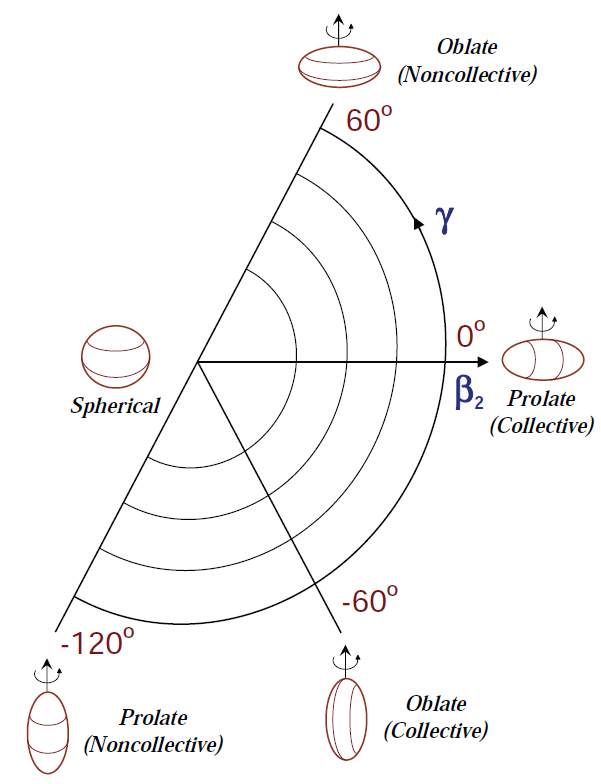
\includegraphics[height=0.25\textheight]{./img/c2/lundconv.png}}
	\caption{Schematic of the Lund convention. Figure adapted from: Ref. \cite{danielDissertation}.}
\end{figure}
\subsection{The Nilsson Model}
To correct the shell model's deficiencies in treating deformed nuclei, in 1955 S.G. Nilsson introduced a modified version of the shell model in Ref \cite{nilsson}. Often called the Nilsson Model, this modified shell model allows deformation to be taken into account using an anisotropic harmonic oscillator potential as follows:
\begin{equation}
\label{eqn:chp2-nilsson-hamil}
H_{nil}=-\frac{\hbar^{2}}{2m}\nabla^{2} + \frac{m}{2}\left(\omega_{x}^{2}x^{2} + \omega_{y}^{2}y^{2} + \omega_{z}^{2}z^{2}\right) + 2\kappa \hbar \omega_{o}\left[\vec{l}\cdot \vec{s} - \mu \left(l^{2} - \left \langle l^{2} \right \rangle_{N} \right) \right]
\end{equation} 
Here $\omega_{x,y,z}$ are the oscillator frequencies in each of the three dimensions, $\kappa$ controls the strength of the spin orbit, and $\mu$ controls the strength of the correction term. The correction term $l^2 - \left \langle l^{2} \right \rangle_{N}$ originally had the form of $\mu l^2$ \cite{nilsson}. It served the purpose of supressing the energy of the higher lying shells, however it was noted in Ref. \cite{nilssonCorrection} that this shift was to large for large N quantum numbers and so the correction term was modified to its current form to compensate. The three oscillator frequencies are chosen to be inversely proportional to the axis lengths of the ellipsoid $a_x$, $a_y$, and $a_z$ as follows:
\begin{align}
\label{eqn:chp2-nilsson-oscilator-freq}
\omega_i = \omega_0\frac{R_0}{a_i} &  & i=x,y,z
\end{align}
Here $\omega_0$ is the oscillator frequency for the spherical case, defined as $\hbar\omega_0 = (\omega_x \omega_y \omega_z )^{1/3}$. In the case of axial symmetry the oscillator frequencies are defined in terms of the deformation parameter $\epsilon_2$ as follows.
\begin{align}
\label{eqn:chp2-nilsson-oscilator-freq-components}
\omega_{x}=\omega_{y}=\omega_{\bot}&=\omega(\epsilon_2)\left(1+\frac{1}{3}\epsilon_2 \right)\\
\omega_{z}=\omega_{\parallel}&=\omega(\epsilon_2)\left(1-\frac{1}{3}\epsilon_2 \right)\\
\omega(\epsilon_2) &= \omega_0\left(1-\frac{1}{3}\epsilon_2^2-\frac{2}{27}\epsilon_2^3\right)^{-1/6}
\end{align}
Here the deformation $\beta$ is defined with respect to $\epsilon_2$ using the following series:
\begin{align}
\label{eqn:chp2-nilsson-beta-from-epsilon}
\beta = \sqrt{\frac{16 \pi}{5}}\left( \frac{1}{3}\epsilon_2 + \frac{1}{9}\epsilon_2^2 + \frac{1}{27}\epsilon_2^3 +  \frac{1}{81}\epsilon_2^4...\right)
\end{align}

With these definitions and the Nilsson Hamiltonian the energy eigenstates ($\epsilon_{\Omega[Nn_z\Lambda]}$), sometimes called Nilsson orbitals can be extracted from solving the Sch\"odinger equation.
\begin{equation}
\label{eqn:chp2-schodinger-eqn-nilsson}
H_{nil}\psi_{i}=\epsilon_{i}\psi_{i}
\end{equation}
Here $i$ represents the complete set of asymptotic quantum numbers used to specify Nilsson orbitals:
\begin{equation}
\label{eqn:chp2-nilsson-numbers}
\Omega^{\pi}[Nn_z\Lambda]
\end{equation}
$\Omega$ is projection of the particle's total angular momentum onto the symmetry axis, $\pi$ is the parity defined as $\pi=(-1)^{l}=(-1)^{N}$, $N$ is the oscillator quantum number, $n_z$ is the number of oscillator quanta (number of nodes in the wavefunction), and $\Lambda$ is the projection of the particle's orbital angular momentum onto the symmetry axis. Some of these quantum numbers are shown schematically in Fig. \ref{fig:chp2-nillson-qn}. 

\begin{figure}[hb!]
\centerline{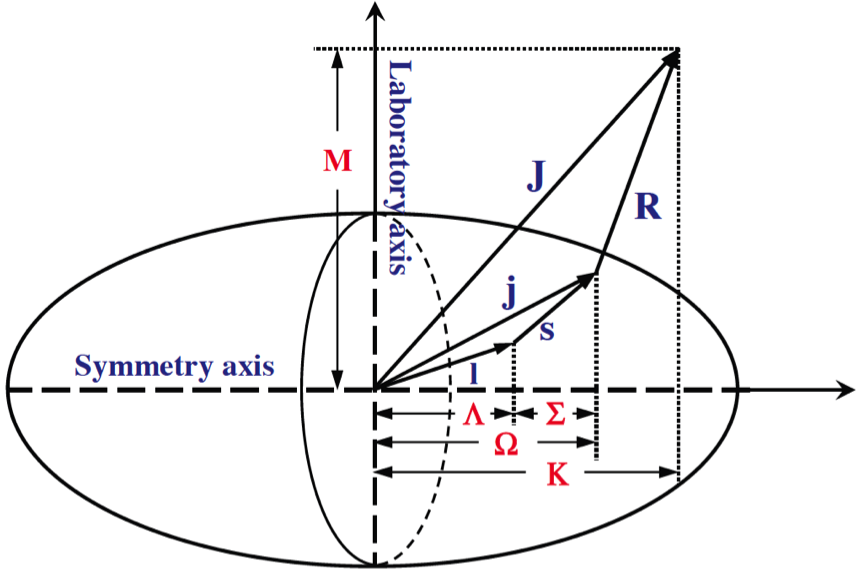
\includegraphics[height=0.22\textheight]{./img/c2/nilsondescr.png}}
	\caption{Schematic of an axially symmetric nucleus and the various quantum numbers that are used in the description of the system. Here R is the angular momentum of collective rotation, J is the total nuclear angular momentum, j is the total angular momentum of the particle, l is the orbital angular momentum of the particle, s is the spin of the particle, M is the projection of J onto the non-symmetry axis, K is the projection of J onto the symmetry axis, $\Omega$ is the projection of j onto the symmetry axis, $\Lambda$ is the projection of l onto the symmetry axis, and $\Sigma$ is the projection of s onto the symmetry axis. Figure adapted from: Ref. \cite{danielDissertation}.\label{fig:chp2-nillson-qn}}
\end{figure}

The deformation dependence of Nilsson orbitals is usually summarized in a Nilsson diagram. In these diagrams energy levels for various sets of asymptotic quantum numbers are plotted versus the deformation parameter $\epsilon$. A Nilsson diagram for protons in the $40\leq{}Z\leq82$ region is shown in Fig. \ref{fig:chp2-nillson-protons}. A diagram for neutrons in the $40\leq{}Z\leq82$ region is shown in Fig. \ref{fig:chp2-nillson-neutrons}. Together these diagrams cover the $A\sim 130$ region where \pr{} lies.

\begin{figure}[h!]
\centerline{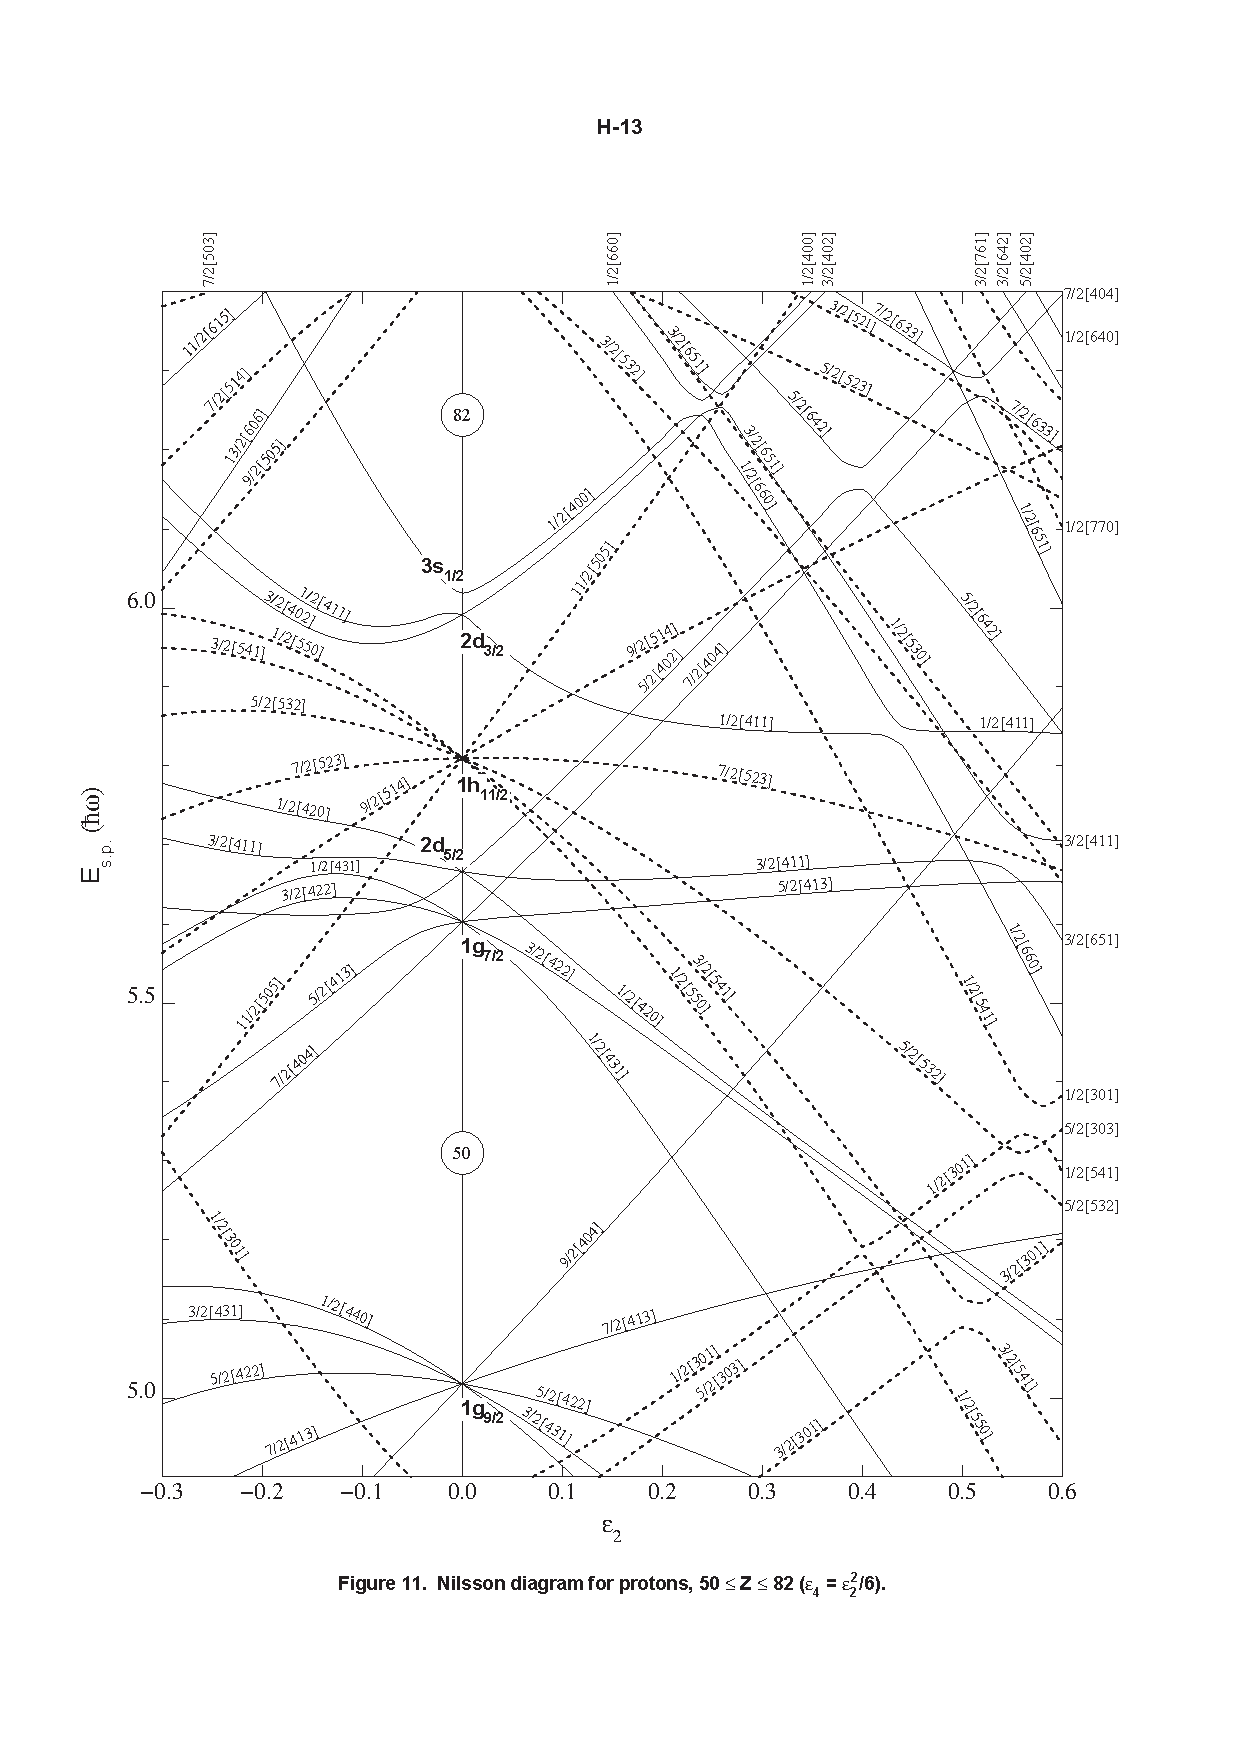
\includegraphics[height=0.8\textheight,clip=true,trim=10 100 10 100]{./img/c2/nilsson_proton_diagram.pdf}}
	\caption{Nilsson diagram for protons in the $50\leq Z \leq 82$ region with $\epsilon_4=\epsilon_2/6$. Solid lines represent positive parity orbitals and dashed lines represent negative parity orbitals. Labels follow the $\Omega$[N $n_z$ $\Lambda$] convention. Figure adapted from: Ref. \cite{nilssonDiagrams}.\label{fig:chp2-nillson-protons}}
\end{figure}

\begin{figure}[h!]
\centerline{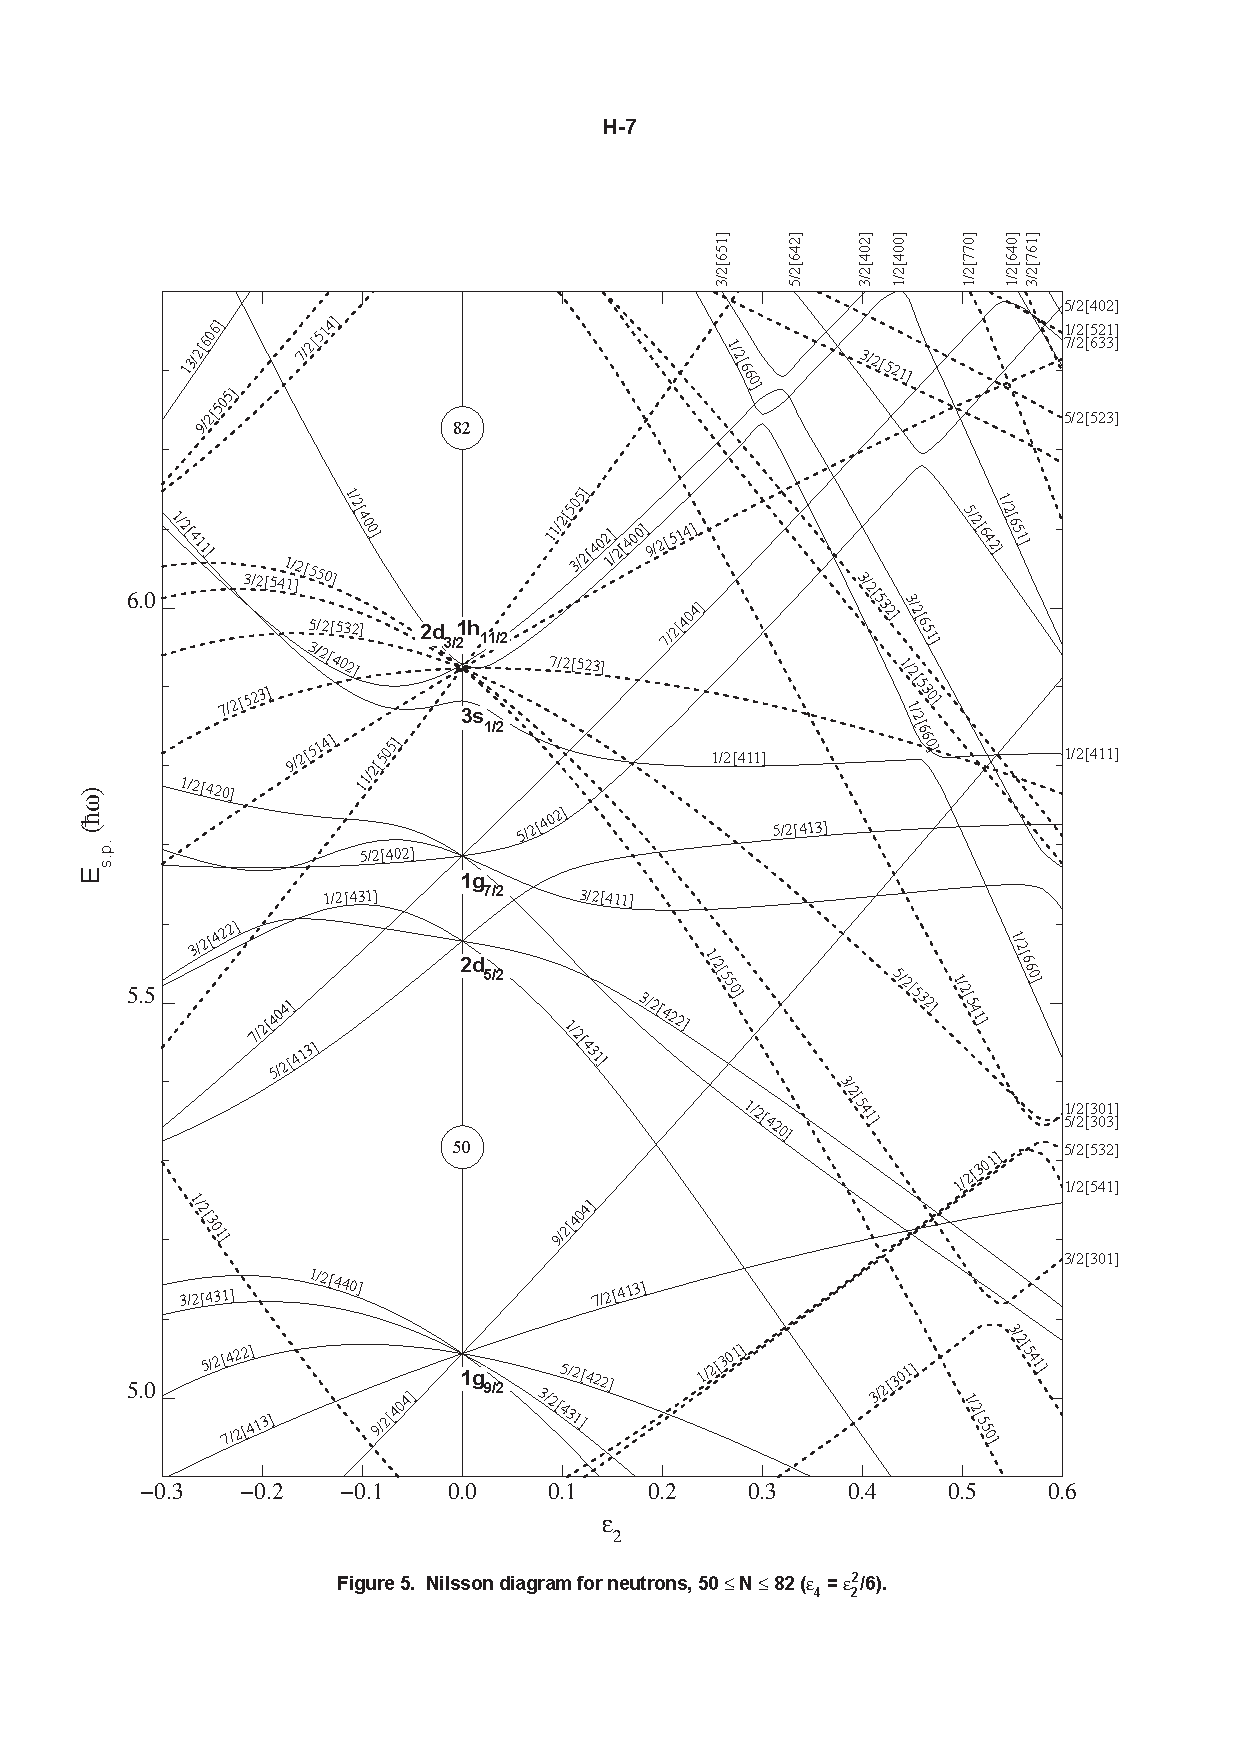
\includegraphics[height=0.8\textheight,clip=true,trim=10 100 10 100]{./img/c2/nilsson_neutron_diagram.pdf}}
	\caption{Nilsson diagram for neutrons in the $50\leq N \leq 82$ region with $\epsilon_4=\epsilon_2/6$. Solid lines represent positive parity orbitals and dashed lines represent negative parity orbitals. Labels follow the $\Omega$[N $n_z$ $\Lambda$] convention. Figure adapted from: Ref. \cite{nilssonDiagrams}.\label{fig:chp2-nillson-neutrons}}
\end{figure}

\section{Collective Rotation}
\label{sec:models-rigid-rotor}
A model of collective nuclear motion was developed by Bohr and Mottleson \cite{bohrMottelson2,bohrMottelsonArticle} due to several observations that could not be explained with single particle motion. Among these are: \emph{1.} Fission, many of the features of which are successfully explained with the liquid drop model \cite{meitnerFissionProducts,fissionMechanism}. \emph{2.} Deformation of the nuclear surface by particle structure \cite{deformationPrediction} giving rise to quadrupole moments which exceed single particle estimates in many nuclei \cite{casimirQuadMoments,nuclearQuadMomentsAndShellStruc}. \emph{3.} The occurrence of electric quadrupole \gr{} transitions with lifetimes much shorter than single particle estimates \cite{nuclearIsomerClassification} which is a characteristic feature of the excitation spectra of strong deformed nuclei \cite{QuadIsomerInterp}.
\subsection{Rigid Triaxial Rotor}
\label{sec:models-triaxial-rotor}
One of the simplest forms of excitation a nucleus can experience is rotation. However, in quantum mechanics, rotation is can only occur about axes that are not symmetry axes (where the symmetry axis is denoted the $\uvec{z}$-axis. This is because the wave function that describes this system is an eigenfunction of $\uvec{J}_z$, and thus, is symmetrical about the $\uvec{z}$-axis. Due to its symmetrically any rotation of this wave function about the symmetry axis generates only phase shift and has a wave function identical to that of the ground state. Thus, a system cannot collectively rotate about symmetry axes. As spherical nuclei are symmetric about all axes, they cannot exhibit collective rotation at all.

In rotating nuclei there are two primary components of the angular momentum. The first is the rotational angular momentum, $\vec{R}$, generated by the collective motion of many nucleons about some axis. The second component is found when there are unpaired valence nucleons. In these cases their angular momentum, $\vec{j}$, must be accounted for as well. This yields a situation like that in Figure \ref{fig:chp2-nillson-qn} which schematically illustrates the total angular momentum of the nucleus, $\vec{J}$, as the sum of $\vec{R}$ and $\vec{j}$.

While it is often the case that the shape (and thus the moments of inertia (MOI)) of a nucleus change somewhat as spin increases accounting for this can be quite difficult. By approximating the system as a rigid rotor with unchanging MOI the problem can be simplified dramatically while maintaining descriptive power. Here each axis has a fixed MOI and the rotational component of the Hamiltonian depends only on the MOIs and the components of the spin along each axis. In the case of a triaxial nucleus with no unpaired valence particles, (thus $\vec{J}=\vec{R}$) the Hamiltonian can be written as follows \cite{triaxRotorSol,wobblingGeometry}:
\begin{align}
\label{eqn:chp2-triaxial-rotor-hamiltonian}
H &= H_{rot} + H_{intr} \\
H_{rot}&=A_3\uvec{J}_3^2 + A_1\uvec{J}_1^2 + A_2\uvec{J}_2^2
\end{align}
Here $H_{intr}$ is the intrinsic component of the Hamiltonian accounting for the internal state of the nucleus, $A_i = \frac{\hbar^2}{2 \mathcal{J}_i}$ where $\mathcal{J}_i$ is the MOI of rotation about the $i^{th}$ axis, and $\uvec{J}_i$ is the operator for the component of the angular momentum along the $i^{th}$ axis. Rewriting the rotational Hamiltonian to a form that uses the operators $\uvec{J}^2$, $\uvec{J}^2_3$, and $\uvec{J}^2_{\pm}$ yields:
\begin{align}
\label{eqn:chp2-triaxial-rotor-hamiltonian-rewrite}
H_{rot}=& H_{r}^{Diag} + H_{r}^{OffDiag}\\
H_{rd}=&\left[\frac{1}{2}\left(A_1+A_2\right)\uvec{J}^2 + \left(A_3-\frac{1}{2}\left(A_1+A_2\right)\right)\uvec{J}^2_3\right]\nonumber\\
H_{r}^{OffDiag}=&\frac{1}{4}\left(A_1-A_2\right)\left(\uvec{J}^2_++\uvec{J}^2_-\right) \nonumber
\end{align}
Here $H_{r}^{Diag}$ is the diagonal component of the Hamiltonian, $H_{r}^{OffDiag}$ is the off diagonal component, $\uvec{J}^2$ is the total angular momentum operator, and $\uvec{J}^2_{\pm}$ are the angular momentum raising and lowering operators $\uvec{J}_{\pm} = \uvec{J}_1\pm\mathit{i}\uvec{J}_2$. Taking the basis states of the wave function to be \cite{triaxRotorSol}:
\begin{equation}
\label{eqn:chp2-triaxial-rotor-basis}
\Ket{IMK}= \sqrt{\frac{2I+1}{16\pi^{2}(1+\delta_{K0})}} \left[\mathcal{D}^{J}_{MK} + (-1)^J \mathcal{D}^{J}_{-KM}\right]
\end{equation}
Where $\delta_{K0}$ is the Kronecker delta function and $\mathcal{D}^{J}_{MK}$ are the Wigner D-functions which are functions of the three Euler angles that determine the orientation of the nucleus' principal axes in space. With these basis states the diagonal portion of the Hamiltonian matrix are:
\begin{equation}
\label{eqn:chp2-triaxial-diagonal-hamil}
\Bra{IMK}H_{rot}\Ket{IMK}=\frac{1}{2}\left(A_1+A_2\right)\left(J(J+1)-K^2\right) + A_3K^2
\end{equation}
Similarly the off diagonal components are:
\begin{equation}
\label{eqn:chp2-triaxial-offdiagonal-hamil}
\Bra{IMK}H_{rot}\Ket{IMK\pm{}2}=\frac{1}{4}\left(A_1-A_2\right)\sqrt{(I\mp{}K)(I\pm{}K+1)(I\mp{}K-1)(I\pm{}K+2)}
\end{equation}
With these, finding the energy eigenvalues and eigenstates for a given spin I is a matter of diagonalizing the matrix. The reduced transition probabilities for $E2$ transitions of the triaxial rotor model are given by \cite{wobblingGeometry}:
\begin{align}
\label{eqn:chp2-triaxial-rotor-reduced-transitions}
B\left(E2,I\rightarrow{}I'\right) &=\sum\limits_{\mu{},K,K'}^{}|\Bra{I'M'K'}\mathcal{M}^E_{2\mu}\Ket{IMK}|^2\\
\mathcal{M}^E_{2\mu} &= \sqrt{\frac{5}{16\pi}}\left[\mathcal{D}^{2*}_{\mu{}0}\uvec{Q}'_{20}+\left(\mathcal{D}^{2*}_{\mu{}2}+\mathcal{D}^{2*}_{\mu{}-2}\right)\uvec{Q}'_{22}\right] \nonumber\\
Q'_{20} &= Q Cos(\gamma) ~~~~~~~ Q'_{22} = \frac{1}{\sqrt{2}}Q Sin(\gamma) \nonumber
\end{align}

\section{Pairing}
The pairing interaction is the force that couples two identical nucleons in time reversed orbits (opposite spin projections). Evidence for this force can be seen in a variety of experimental results. Among them: 1) The staggering seen in the single neutron (or proton) separation energies between even and odd neutron (or proton) number (see Fig. \ref{fig:chp2-s1n-staggering}). 2) The ground state of \emph{every} even-even nucleus has $J^{\pi}=0^+$. 3) The ground states of the odd-A nuclei always have $J^{\pi}$ determined by the orbital of the last unpaired nucleon.

\begin{figure}[t!]
\centerline{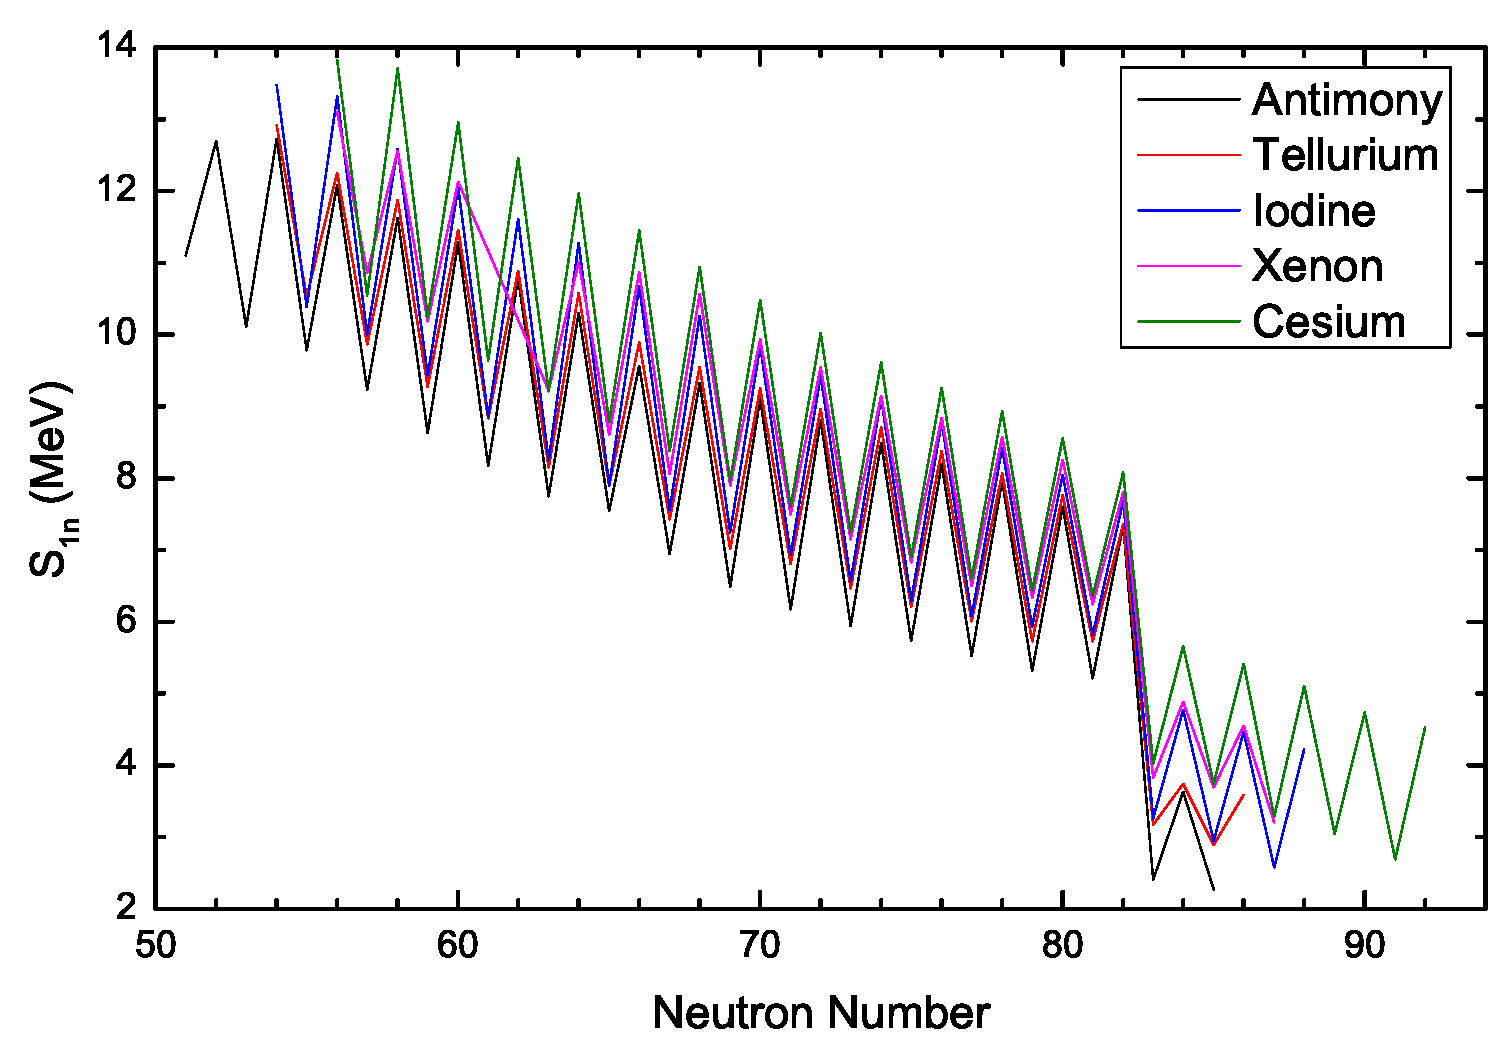
\includegraphics[height=0.3\textheight]{./img/c2/S1n_MassChains.eps}}
	\caption{One neutron separation energies vs neutron number for the five isotopes from $Z=51$ to $Z=55$. The staggering between even and odd masses gives strong evidence for the pairing interaction. Additionally the $N=82$ shell gap can be seen. Figure adapted from: Ref. \cite{nilssonDiagrams}.\label{fig:chp2-s1n-staggering}}
\end{figure}

M. Goeppert gave the first theoretical tool to calculate this interaction in 1950 \cite{pairingFirstTheory} describing the pairing force as a delta function multiplied by some interaction strength.
\begin{equation}
\label{eqn:chp2-pairing-first-function}
V_{pair}=-G\delta(\phi_1-\phi_2)\delta(Cos(\theta_1)-Cos(\theta_2))\frac{\delta(r_1-r_2)}{r^2}
\end{equation}
Here $\delta(x)$ is the Dirac delta function and g is the pairing interaction strength. Calculations were performed using this interaction to explore its effects \cite{pairingCorrEffectOnProperties} and then later analogies between nuclear pairing and BCS superconductivity theory were discovered and explored \cite{pairingAnalogyToBCS,pairingSuperfluidity,bcsTheory}. The pairing strength $G$ has been determined to have different values for the protons and neutron. For protons the pairing strength is approximately $G_p=\sfrac{17}{A} MeV$ and for neutrons the pairing strength is approximately $G_p=\sfrac{23}{A} MeV$. This result is expected given the repulsive interaction between protons which works counter to the pairing force. The expectation value for this interaction is:
\begin{equation}
\label{eqn:chp2-pairing-expectation}
\Braket{j_1j_2J|V_{pair}|j3j4J'}=-G\sqrt{\left(j_1+\sfrac{1}{2}\right)\left(j_3+\sfrac{1}{2}\right)}\delta_{j_1j_2}\delta_{j_3j_4}\delta_{J0}\delta_{J'0}
\end{equation}
In the second quantization formalism the pairing Hamiltonian is usually written in the form:
\begin{equation}
\label{eqn:chp2-pairing-hamil}
H_{pair} = -GP^+P-\lambda{}\uvec{N}
\end{equation}
Where $P^+$ and $P$ are the pair creation and annihilation operators, $\lambda$ is the chemical potential, and $\uvec{N}$ is the particle number operator.

If the spacing between levels near the Fermi surface is small relative to $G$ then the pairing interaction scatters pairs of nucleons with $J^{\pi}=0^+$ from occupied levels to empty levels above the Fermi level. This results in the ``smeared'' nucleon distribution shown in the dashed line of Fig. \ref{fig:chp2-pairing-fermi-surface}. If the level spacing is large near the Fermi surface then the pairing interaction cannot scatter pairs into unoccupied levels and the Fermi surface has a sharp cutoff as seen in the solid line of Fig. \ref{fig:chp2-pairing-fermi-surface}.
\begin{figure}[t!]
\centerline{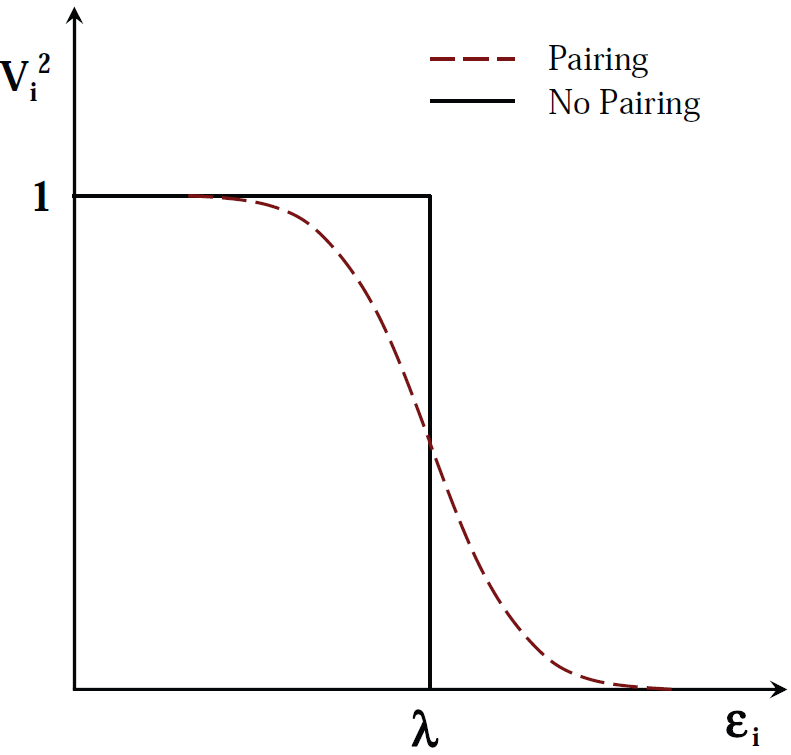
\includegraphics[height=0.3\textheight]{./img/c2/pairinginteraction.png}}
	\caption{Schematic of the occupancy of single particle states with and without pairing. Figure adapted from: Ref. \cite{xfwangDissertation}.\label{fig:chp2-pairing-fermi-surface}}
\end{figure}

The energy range that this ``smearing'' of level occupancies covers is equal to the gap parameter ($\Delta$) which can be defined as follows:
\begin{equation}
\label{eqn:chp2-pairing-gap-param}
\Delta = G\sum\limits_{ij}^{}U_iV_j
\end{equation}
Where $U$ is the emptiness factor (the probability that a state will be occupied by a hole) and $V$ is the fullness factor (the probability that a state will be occupied by a particle. $U$ and $V$ are defined as follows
\begin{align}
\label{eqn:chp2-pairing-gap-param-defs}
V_i &= \sqrt{\frac{1}{2}\left(1+\frac{\epsilon_1-\lambda}{\sqrt{(\epsilon_1-\lambda)^2+\Delta^2}}\right)}\\
U_i &= \sqrt{\frac{1}{2}\left(1-\frac{\epsilon_1-\lambda}{\sqrt{(\epsilon_1-\lambda)^2+\Delta^2}}\right)}
\end{align}
Here $\epsilon_i$ represents the single particle energies, and $\lambda$ is the chemical potential for a given number of particles. The probabilities are normalized such that $U_i^2+V_i^2=1$. Far below the Fermi surface the probability that an orbit will be occupied is $V_i=1$ while the probability that the orbit is unoccupied $U_i=0$. This situation reverses itself far above the Fermi surface. Close to the Fermi surface both probabilities will have a finite value. BCS theory \cite{bcsTheory} tells us that the quasiparticle energy is expressed by:
\begin{equation}
\label{eqn:chp2-pairing-qp-en}
E_{qp}(n,p)=\sqrt{(\epsilon_i-\lambda)^2+\Delta^2}
\end{equation}

As the nucleus rotates the induced Coriolis force competes with the pairing interaction. This competition attempts to break the pairs and align the individual angular momenta of the nucleons with the rotation axis. In general rotational motion weakens the pairing strength in the nucleus. While some pairs break and align at specific rotational frequencies, all pairs will feel the effects. This phenomenon is called the Coriolis anti-pairing effect (CAP) \cite{bohrMottelsonRotationWeakensPairing}.

\section{Quasiparticle + Triaxial Rotor (QTR)}
\label{sec:models-qtr}
The QTR model is an extension of the particle + rotor model which was put forth in its most primitive form in 1952 by Aage Bohr in Ref. \cite{bohrParticlePlusRotor}. This model allows the calculation of the effect of coupling the odd quasiparticle to the triaxial even-even core. The Hamiltonian of this model is given in Ref. \cite{frauendorfTransverseWobbling} to be:
\begin{align}
\label{eqn:chp2-qtr-hamil}
H&=H_{sqp}+H_{rot}-H_{int}\\
H_{rot}&=A_3(\uvec{J}_3-\uvec{j}_3)^2+A_1(\uvec{J}_1-\uvec{j}_1)^2+A_2(\uvec{J}_2-\uvec{j}_2)^2\\
H_{int}&= \sum\limits_{\mu}^{}q^*_{\mu}Q_{\mu} = f r^2 \left(\epsilon Cos(\gamma) \bar{Y}^2_0 + \frac{\epsilon Cos(\gamma)}{\sqrt{2}}\left(\bar{Y}^2_2 + \bar{Y}^2_{-2}\right)\right)
\end{align}
Here $H_{sqp}$ is the single quasiparticle Hamiltonian accounting for the presence of the central potential and the pairing interaction, $H_{rot}$ is the rotor model Hamiltonian, $H_{int}$ is the interaction of the quasiparticle to the triaxial core, $\uvec{J}_k$ is the total angular momentum of the system along the $k^{th}$ axis, $\uvec{j}_k$ is the angular momentum of the quasiparticle along the $k^{th}$ axis, $\bar{Y}^l_m$ is the result of applying the spherical harmonic operator $Y^l_m$ to the basis state, and $f$ is a scaling factor obtained in the following manner:
\begin{align}
\label{eqn:chp2-qtr-int-hamil-scaling}
\kappa f &= \frac{2}{3}\sqrt{\frac{4\pi}{5}}\hbar\omega_{\circ}\\
\kappa \Bra{0}|Q|\Ket{2} & = \hbar\omega_{\circ} \epsilon Cos(\gamma)
\end{align}
Here $\Bra{0}|Q|\Ket{2}$ is the reduced matrix element of the core quadrupole operator between the  $0^+$ ground state and the first $2^+$ state. This is related to the reduced quadrupole transition probability as follows:
\begin{equation}
\label{eqn:chp2-red-mat-el-to-red-trans-prob}
B(E2,J_I\rightarrow{}J_F)=\frac{|\Bra{J_F}|Q|\Ket{J_I}|^2}{2J_I+1}
\end{equation}

Qualitatively, the $H_{int}$ works as follows. A high j quasiparticle with predominantly particle nature will align its $\vec{j}$ to the short axis of the core. This orientation results in the maximum overlap of the torus-like density distribution of the quasiparticle and the triaxial core which minimizes the energy of the attractive interaction between the two. For a high j quasiparticle with hole nature the $\vec{j}$ aligns to the long axis which minimizes the overlap of the torus with the triaxial core which in turn minimizes the energy of the repulsive interaction between the two. Finally a quasiparticle from the middle of the shell, possessing particle and hole nature in roughly equal measure would align the medium axis of the triaxial core.

The reduced transition probabilities of this system can be extracted in a manner similar to that in the triaxial rotor model (equation \ref{eqn:chp2-triaxial-rotor-reduced-transitions}) however the operator $\mathcal{M}^E_{2\mu}$ will change to account for the quadrupole moment of both the core ($Q$) and the quasiparticle ($q$).

\section{Tilted Axis Cranking}
\label{sec:models-tac}
The tilted axis cranking (TAC) model \cite{frauendorfTAC} is a generalization of the cranked shell model introduced by Inglis in 1954 \cite{crankedShellModel}. In this model, nucleons are individual particles independently moving in an average potential, which in turn rotates about some axis. As expected of a rotating frame, the Coriolis and centrifugal forces play an important role in the TAC model with consequences for shape and pairing correlations. The Hamiltonian for this model has two terms, the cranking component $-\omega\uvec{J}_x$ which represents the centrifugal and Coriolis forces from the rotating reference frame and a component in the rotating frame, $H_0$.
\begin{equation}
\label{eqn:chp2-TAC-Hamiltonian}
H'=H_0-\omega\uvec{J}_x
\end{equation}
If the deformation is small and quadrupole nature the component in the rotating frame is given in Ref. \cite{frauendorfTAC} to be:
\begin{equation}
\label{eqn:chp2-TAC-invar-Hamiltonian}
H_0=H_{sph}-\frac{\chi}{2}\sum\limits_{\mu=-2}^{2}Q_{\mu}^+Q_{\mu} - GP^+P-\lambda\uvec{N}
\end{equation}
Here the spherical potential is simply parameterized as by the energy $\epsilon_k$ for a state labeled $k$ and then constructed in second quantization to be:
\begin{equation}
\label{eqn:chp2-TAC-spherical}
H_{sph}=\sum\limits_{k}^{}\epsilon_kc^+_kc_k
\end{equation}
The short range pair correlations are accounted for using the monopole pair operator:
\begin{equation}
\label{eqn:chp2-TAC-pairing}
P^+=\sum\limits_{k>0}^{}c^+_kc^+_{\bar{k}}
\end{equation}
Here $\bar{k}$ represents the time reversed state of $k$, \emph{i.e.} spin-up $\rightarrow$ spin-down. The quadrupole interaction operator accounts for the long range particle-hole interaction:
\begin{equation}
\label{eqn:chp2-TAC-quad}
Q_{\mu}=\sum\limits_{k,k'}^{}\sqrt{\frac{4\pi}{5}}\Bra{k}r^2Y_{2\mu}\Ket{k'}c^+_kc_{k'}
\end{equation}
Finally, the term $\lambda\uvec{N}$ accounts for the number of particles (N) using the chemical potential $\lambda$. As written the Hamiltonian of equation \ref{eqn:chp2-TAC-Hamiltonian} only accounts for one type of particles, protons or neutron, thus in all the expressions should be understood as sums across neutron and proton parts.

To determine the system wave functions,  $\ket{}$, the eigenstates of the Hartree-Fock-Bogoliubov (HFB) are determined. In the adiabatic limit, where it is assumed that the frequency of intrinsic motion is large compared to the frequency of rotation, the HFB Routhian is:
\begin{equation}
\label{eqn:chp2-TAC-HFB-Routhian}
h'=h - \sum\limits_{\mu=-2}^{2}(q_{mu}Q^+_{\mu}+q^*_{mu}Q_{\mu}) - \Delta(P^++P) - \lambda{}N-\omega\uvec{J}_z
\end{equation}
Applying the self-consistency conditions: $q_{\mu}=\chi{}\braket{Q_{\mu}}$, $\Delta=G\braket{P}$, and conservation of particle number $N=\braket{\uvec{N}}$ gives the deformed potential $h$. For further information regarding operator definitions and procedures for self-consistent solutions can be found in References: \cite{frauendorfTACMultiQPBands,frauendorfTAC,nuclearManyBodyProblem}

As stated in Refs. \cite{frauendorfTACMultiQPBands,timeDepVarMethodForRotation}, self consistent solutions must have their angular frequency and angular momentum vectors be parallel \emph{i.e.} $\vec{\omega}\parallel\vec{J}$. Additionally, self consistent solutions to the total Routhian ($E'=\braket{H'}$) satisfy the extremum conditions of:
\begin{equation}
\label{eqn:chp2-tac-extrema-cond}
\left. \frac{\partial{}E'}{\partial{}q_{\mu}} \right|_{\omega}=0 ~~~~~ \left. \frac{\partial{}E'}{\partial{}\Delta} \right|_{\omega}=0
\end{equation}
and have total energy and angular momentum:
\begin{align}
E(J)=E'(\omega)+\omega{}J(\omega) & & J(\omega) = \braket{\uvec{J}_z}
\end{align}

The orientation intrinsic frame is chosen such that the components of the quadrupole tenser satisfy $q'_{-1}=q'_1=0$ and $q'_{-2}=q'_2$. With this the principal axes of the intrinsic frame coincide with the principal axes of the quadrupole tensor and both are related to the lab frame by the three Euler angles $\psi$, $\theta$, and $\phi$, shown in Fig. \ref{fig:chp2-TAC-euler-angles}. The component quadrupole moments of the lab frame, $q_{\mu}$, are related to the quadrupole moments of the intrinsic frame, $q_{\mu}'$, as follows:
\begin{equation}
\label{eqn:chp2-intrin-quad-to-lab-quad}
q_{\mu} = \mathcal{D}^2_{\mu{}0}(\psi,\theta,\phi)q'_0+\left[\mathcal{D}^2_{\mu{}2}+\mathcal{D}^2_{\mu{}-2}(\psi,\theta,\phi)(\psi,\theta,\phi)\right]q'_2
\end{equation}
With the intrinsic quadrupole moments expressed using the standard deformation parameters of the Lund convention:
\begin{equation}
\label{eqn:chp2-lund-conv-quad-moments}
q'_0=K\beta{}*Cos(\gamma) ~~~~~~~~~~~ q'_2 = -K\frac{\beta{}Sin(\gamma)}{\sqrt{2}}
\end{equation}
where $K$ sets the energy scale for the deformed potential \cite{frauendorfTAC}.
\begin{figure}[t!]
\centerline{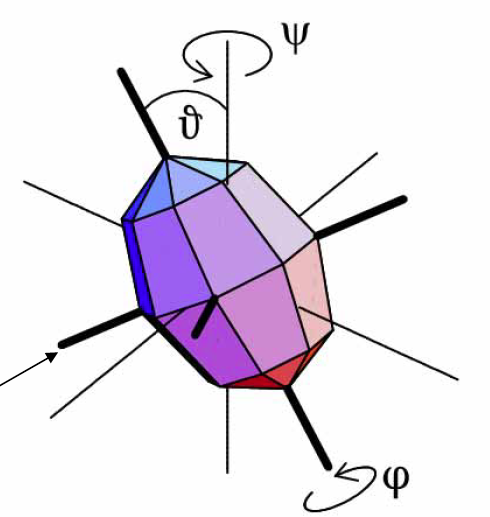
\includegraphics[height=0.3\textheight]{./img/c2/tiltorientation.png}}
	\caption{Orientation of the rotational axis with respect to the principal axes of the deformed density distribution. Figure taken from: Ref. \cite{danielDissertation}.\label{fig:chp2-TAC-euler-angles}}
\end{figure}

As the rotation angle $\psi$ is about the cranking axis the intrinsic states are invariant with respect to it and it is set to zero. With this, in the intrinsic frame, the mean-field Routhian is fixed by $\beta$, $\gamma$, $\theta$, and $\phi$, the two parameters of the deformation and the two parameters of the orientation of $\vec{\omega}$ relative to the principal axes. If we take the angular velocity as:
\begin{equation}
\label{eqn:chp2-ang-vel-vec}
\vec{\omega}=(\omega_1,\omega_2,\omega_3)=\omega(Sin(\theta)Sin(\phi),Sin(\theta)Cos(\phi),Cos(\theta))
\end{equation}
then the HFB Routhian becomes:
\begin{align}
\label{eqn:chp2-TAC-HFB-intrin-routh-rewrite}
h'=h& -q'_0Q'_0-q'_2(Q'_2+Q'_{-2})-\Delta(P^++P)-\lambda\uvec{N} \\
&- \omega(J_1Sin(\theta)Sin(\phi)+J_2Sin(\theta)Cos(\phi)+J_3Cos(\theta)) \nonumber
\end{align}
With this $\beta$ and $\gamma$ are determined from the self-consistency equations
\begin{equation}
\label{eqn:chp2-TAC-beta-gamma-self-consist}
q'_0=\kappa\Braket{Q'_0}~~~~~~~~~~q'_2=\kappa\Braket{Q'_2}
\end{equation}
The remaining Euler angles $\theta$ and $\phi$ are determined from the self-consistency requirement of $\vec{J}\parallel\vec{\omega}$. These parameter sets correspond to extrema of the total Routhian:
\begin{equation}
\label{eqn:chp2-tac-extrema-cond2}
\left. \frac{\partial{}E'}{\partial{}q'_{0}} \right|_{\omega}=0 ~~~~ \left. \frac{\partial{}E'}{\partial{}q'_{2}} \right|_{\omega}=0 ~~~~ \left. \frac{\partial{}E'}{\partial\theta} \right|_{\omega}=0 ~~~~ \left. \frac{\partial{}E'}{\partial\phi} \right|_{\omega}=0
\end{equation}
Of these extrema, only the minima are interpreted as bands.

Due to the invariance of the intrinsic quadrupole moments $Q'_0$ and $(Q'_2+Q'_{-2})/\sqrt{2}$ with respect to the rotations $\mathscr{R}_1(\pi)$, $\mathscr{R}_2(\pi)$, and $\mathscr{R}_3(\pi)$ restrictions can be placed on the Euler angles as follows: $0\leq\psi\leq{}2\pi$, $0\leq\theta\leq\pi/2$, and $0\leq\phi\leq\pi$. With these restrictions in mind we can see that there are three possible TAC solutions. They are: the axial solution which is shown in top panel of Fig. \ref{fig:chp2-TAC-solution-types}, the planar solution, found in the middle panel of Fig. \ref{fig:chp2-TAC-solution-types}, and finally, the aplanar solution, which is in the bottom panel of Fig. \ref{fig:chp2-TAC-solution-types}. The axial and planar solutions of the TAC model will be discussed in greater depth in the subsequent sections. The aplanar solution, as it is unimportant to the work in this dissertation, will not be discussed further save to say that it gives rise to one of the two unique signatures of nuclear triaxiality, chirality. Ref. \cite{frauendorfTAC} and Ref. \cite{frauendorfChirality} both have very good discussions of this solution and its implications.
\begin{figure}[t!]
\centerline{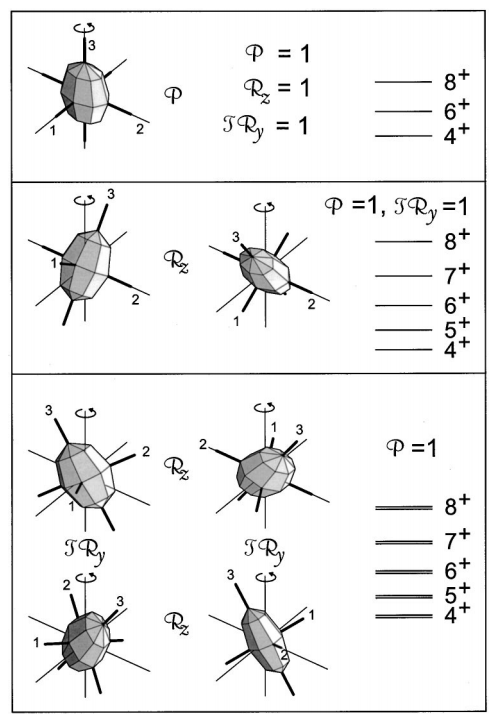
\includegraphics[height=0.6\textheight]{./img/c2/tacsolutions.png}}
	\caption{Discrete symmetries of the mean field of a rotating triaxial nucleus for each of the TAC solutions along with schematics of the band structures that arise from each solution. The axis of rotation ($z$), which coincides with the $\vec{J}$, is marked with a circular arrow. The operators are: $\mathscr{P}$: Parity inversion, $\mathscr{R}_{y,z}$: Rotation by $\pi$ about the $y$ or $z$ axis, and $\mathscr{T}$: Time reversal. Figure adapted from: Ref. \cite{frauendorfTAC}.\label{fig:chp2-TAC-solution-types}}
\end{figure}

\subsection{Rotation About A Principal Axis}
If the axis of rotation, ($z$), coincides with one of the principal axes of the self consistent solution, then the solution is called Principal Axis Cranking (PAC) and the orientation angles satisfy:
\begin{equation}
\label{eqn:chp2-PAC-angle-conditions}
\theta = 0, \sfrac{\pi}{2}~~~~~~~ \phi= 0, \sfrac{\pi}{2}
\end{equation}
The upper panel of Fig. \ref{fig:chp2-TAC-solution-types} shows the PAC case where $\vec{J}$ has the direction of the principal axis 3. In this case the solution has the following properties:
\begin{equation}
\label{eqn:chp2=TAC-PAC-sol-prop}
\mathscr{R}_z(\pi)\Ket{}=e^{-i\alpha\pi}\Ket{}
\end{equation}
Here $\alpha$ is the quantum number called signature. In this situation $\alpha$ is a good quantum number and the values that the total spin take on follow the selection rule:
\begin{equation}
\label{eqn:chp2=TAC-PAC-spin-sel-rule}
I=\alpha+2n ~~~~~n\in{}\mathds{Z}
\end{equation}
This selection rule shows that the PAC solution represents a single $\Delta{}I=2$ band, as is illustrated on the right side of the upper panel of Fig. \ref{fig:chp2-TAC-solution-types}.

\subsection{Rotation About A Tilted Axis}
If the axis of rotation does not coincide with one of the principal axes but still lies within the planes defined by them, then the solution is called the Planar Tilted Axis Cranking (TAC) solution. In this case the orientation angles satisfy:
\begin{align}
\theta &\neq{} 0, \sfrac{\pi}{2} ~~~~~~ \phi=0, \sfrac{\pi}{2}\\
\theta &= 0, \sfrac{\pi}{2} ~~~~~~ \phi\neq{}0, \sfrac{\pi}{2}
\end{align}
This situation in the middle panel of Fig. \ref{fig:chp2-TAC-solution-types} shows a case of this situation where the axis of rotation lies in the principal planes spanned by axes 1 and 3. As shown in the middle panel of Fig. \ref{fig:chp2-TAC-solution-types} invariance with respect to rotation about the z-axis by $\pi$ is lost, yielding:
\begin{equation}
\label{eqn:chp2=TAC-TAC-sol-prop}
\mathscr{R}_z(\pi)\Ket{}\neq{}e^{-i\alpha\pi}\Ket{}
\end{equation}
With the breaking of this symmetry, $\alpha$ ceases to be a good quantum number and there is no longer a selection rule on the total spin. This can be seen schematically on the right side of the middle panel of Fig. \ref{fig:chp2-TAC-solution-types}.

Since 1993 when Frauendorf found a set of self-consistent Hartree-Fock mean-field solutions for uniform rotation about a tilted axis \cite{frauendorfTiltedCranking} TAC has turned out to be a reliable approximation to calculate and investigate the properties of the various types of rotational bands. Details of TAC not covered in this section can be found in Refs. \cite{frauendorfTiltedCranking,frauendorfTACMultiQPBands,frauendorfChirality,frauendorfTAC}

\section{The Wobbling Mode in Nuclei}
\label{sec:models-wobbling}
\subsection{Models of the Wobbling Mode}
The wobbling mode in nuclei was first predicted by Bohr and Mottelson in the second volume of their textbook on nuclear structure \cite{bohrMottelson2}. Their formulation of wobbling was formulated for even even nuclei using only the triaxial rotor model. what is now known as simple wobbling
\subsubsection{Simple Wobbling}
\label{ssec:models-simple-wobbling}
The rotational kinetic energy of the system is:
\begin{equation}
\label{eqn:chp2-rot-kin-en}
E_{rot} = A_3J_3^2 + A_1J_1^2 + A_2J_2^2
\end{equation}
By combining this with the conservation of angular momentum:
\begin{equation}
\label{eqn:chp2-am-cons}
J^3 = J_1^2 + J_2^2 + J_3^2 = I(I+1)
\end{equation}
we can find the classical orbit of $\vec{J}$ at the intersection of the angular momentum sphere and energy ellipsoid. Assuming $A_1>A_2>A_3$ ($\mathcal{J}_1<\mathcal{J}_2<\mathcal{J}_3$) the yrast line then corresponds to the two surfaces touching at $J=J_3$ with rotational energy $E(J)=A_3J^2$. These orbits are illustrated in Figure \ref{fig:chp2-classical-am-orbits}. Here image a is an orbit slightly above the yrast line which is harmonic wobbling motion described by Bohr and Mottelson \cite{bohrMottelson2} (more on this in section \ref{sec:models-wobbling}). Image b is the separatrix, representing
\begin{figure}[t!]
\centerline{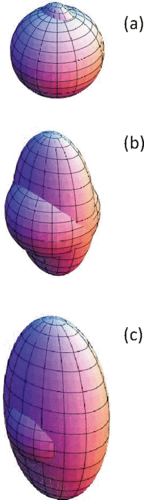
\includegraphics[height=0.25\textheight]{./img/c2/simple_am_orbits.png}}
	\caption{Intersections of the angular momentum and energy surfaces with $A_1=6*A_3$ and $A_2=3A_3$ for $J=2$ taken at progressively larger various energies from a to c. Figure adapted from: Ref. \cite{frauendorfTransverseWobbling}.\label{fig:chp2-classical-am-orbits}}
\end{figure} the unstable rotation about the axis with intermediate MOI, this orbit the boundary between rotation about the axis with the maximum MOI (axis 3) and the axis with minimum MOI (axis 1). Image c gives an example of an orbit corresponding to rotation about axis 1.

\subsubsection{Transverse Wobbling}
\label{ssec:models-transverse-wobbling}
\begin{figure}[t!]
\centerline{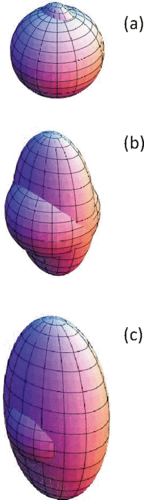
\includegraphics[height=0.25\textheight]{./img/c2/simple_am_orbits.png}}
	\caption{Intersections of the angular momentum and energy surfaces with $A_1=6*A_3$ and $A_2=3A_3$ for $J=2$ taken at progressively larger various energies from a to c. Figure adapted from: Ref. \cite{frauendorfTransverseWobbling}.\label{fig:chp2-transverse-am-orbits}}
\end{figure}

\subsubsection{Longitudinal Wobbling}
\label{ssec:models-long-wobbling}

\subsection{Signatures of Wobbling}
\label{sec:models-sig}
